\documentclass{article}
\usepackage[utf8]{inputenc}
\usepackage[T1]{fontenc}
\usepackage{tikz}
\usepackage{amssymb}

% Blank symbol definition
\newcommand{\blank}{\square}

\usetikzlibrary{automata, positioning, arrows, shapes}

\begin{document}

\begin{center}
\textbf{Decider TM for $L = \{ a^m b^n \mid m \neq n \}$}
\vspace{1cm}

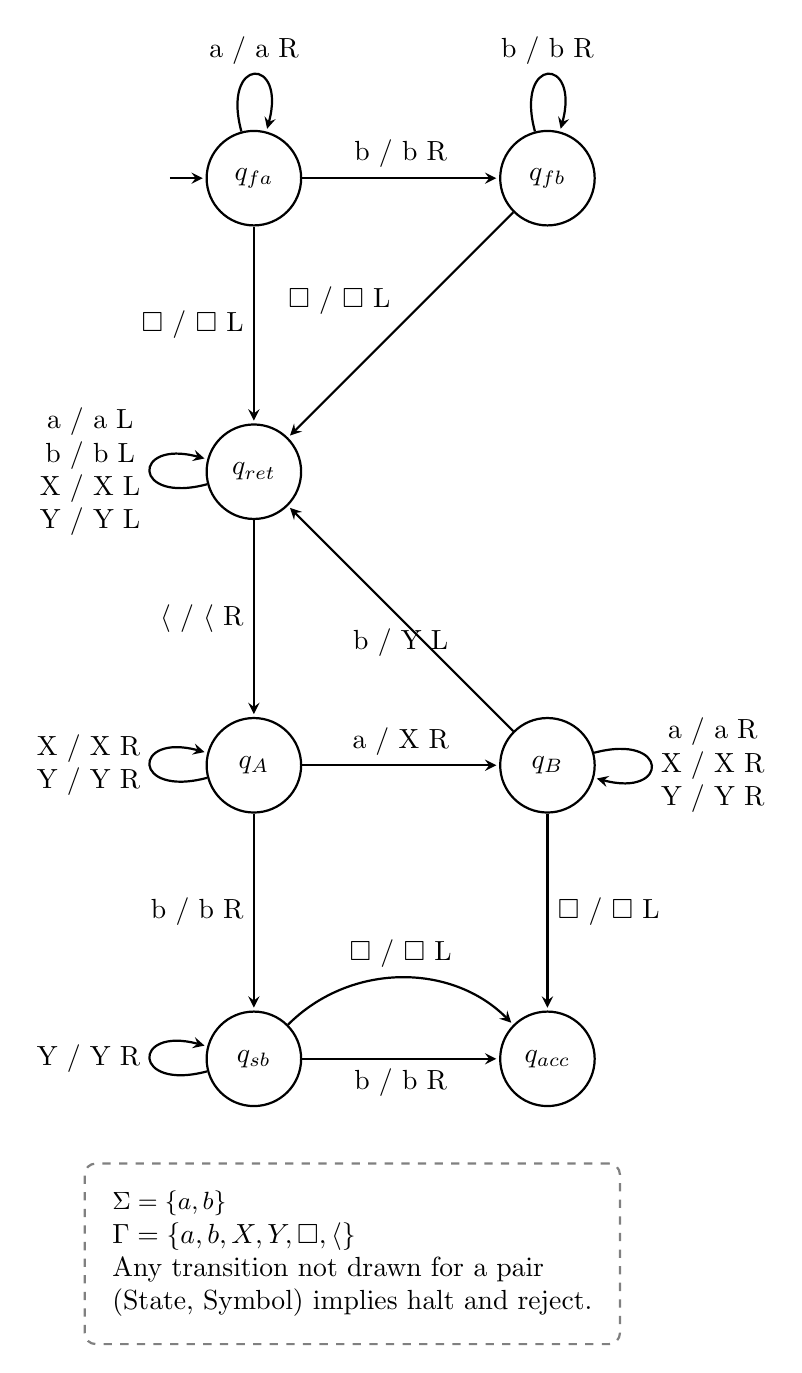
\begin{tikzpicture}[
    ->,
    >=stealth,
    shorten >=1pt,
    auto,
    node distance=2.5cm,
    thick,
    state/.style={circle, draw, minimum size=1.2cm, thick, fill=white},
    accept/.style={double, circle, draw, minimum size=1.2cm, thick, fill=green!10},
    initial text=
  ]

  % --- STATE POSITIONING ---
  \node[state, initial] (qfa) {$q_{fa}$};
  \node[state, right=of qfa] (qfb) {$q_{fb}$};
  \node[state, below=of qfa] (qvol) {$q_{ret}$};
  \node[state, below=of qvol] (qa) {$q_{A}$};
  \node[state, right=of qa] (qb) {$q_{B}$};
  \node[state, below=of qa] (qsb) {$q_{sb}$};
  \node[state, right=of qsb] (acc) {$q_{acc}$};

  % --- TRANSITIONS ---

  % 1. Validation phase
  \path (qfa) edge[loop above] node {a / a R} (qfa)
              edge node {b / b R} (qfb)
              edge node[left] {$\blank$ / $\blank$ L} (qvol);

  \path (qfb) edge[loop above] node {b / b R} (qfb)
              edge node[above left] {$\blank$ / $\blank$ L} (qvol);

  % 2. Return phase
  \path (qvol) edge[loop left] node[align=center] {a / a L \\ b / b L \\ X / X L \\ Y / Y L} (qvol)
               edge node[left] {$\langle$ / $\langle$ R} (qa);

  % 3. Pairing phase A
  \path (qa) edge[loop left] node[align=center] {X / X R \\ Y / Y R} (qa)
             edge[right] node[above] {a / X R} (qb)
             edge node[left] {b / b R} (qsb);

  % 4. Pairing phase B
  \path (qb) edge[loop right] node[align=center] {a / a R \\ X / X R \\ Y / Y R} (qb)
             edge node[below] {b / Y L} (qvol)
             edge[below] node[right] {$\blank$ / $\blank$ L} (acc);

  % 5. Remaining B's check
  \path (qsb) edge[loop left] node {Y / Y R} (qsb)
              edge node[below] {b / b R} (acc)
              edge[bend left=45] node[above] {$\blank$ / $\blank$ L} (acc);

  % --- LEGEND ---
  \node[draw=black!50, dashed, rounded corners, inner sep=10pt, align=left, anchor=north] 
  at (1.25, -12.5) {
    \small
    $\Sigma = \{a, b\}$\\
    $\Gamma = \{a, b, X, Y, \blank, \langle\}$\\
    Any transition not drawn for a pair\\ (State, Symbol) implies halt and reject.
  };

\end{tikzpicture}
\end{center}

\end{document}
